\chapter{Introduction to Discrete Probability}

Occassionally, the voice in your brain will protest:
\begin{quote}
    \textbf{STOP DOING PROBABILITY!} Years of calculating yet no real-life usage on finding an affordable housing in Berkeley!
\end{quote}
But, probability is in fact useful across many other disciplines and purposes. One of the most applicable example in real life is gambling, gacha, as well as several applications of computer science where we work with statistical and probabilistic frameworks to produce efficient models.

What do statements concerning probability look like? It may be of the following forms:
\begin{bindenum}
    \item The average time between system failure is 5 days.
    \item In average, 1 in 1000 students from UC Berkeley lives in an affordable housing.
    \item The probability at which the game character Mr. Game and Watch rolls a 9 on a fair 8-face dice with values 2 to 9 is precisely $\frac{1}{8}$.
\end{bindenum}
And so on.

Implicitly, all statements concern with a \textbf{probability space}: the result of random experiments that we cosntructed or simulated. Therefore, we would greatly benefit from understanding what random experiments are as we come to discuss \textit{probability space} and \textit{sample space}, two ``frames'' upon which the theories of probability depend on.

\section{Random Experiments}
In general, a \textbf{random experiment} consists of sampling $k$ elements from some set $S$ such that $|S| = n \geq k$. \\
The possible outcomes of such experiment are the objects we count.

Here, the four categories of counting situation (ordered or orderless, with or without replacement) also exist in random experiments. The outcome of random experiment is a \textbf{sample point}, where the \textbf{sample space} ($\Omega$) is the set of all possible outcomes of an experiment.

Let us run through an example:
\begin{ln-fig}{The Sample Space of 4 Coin-Tosses}{}
    \begin{center}
        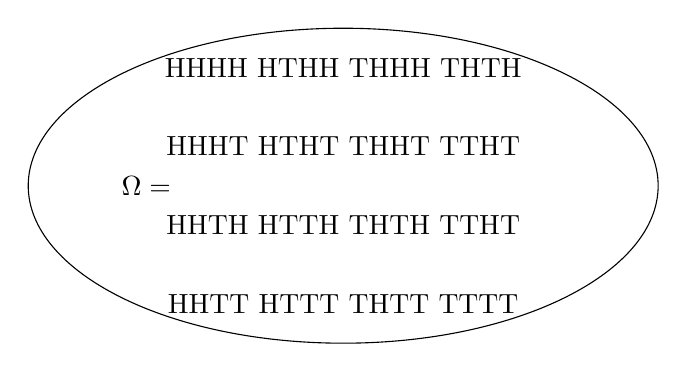
\begin{tikzpicture}
            \draw (0, 0) ellipse (4cm and 2cm);
            \node (eq) at (-2.5, 0) {
                $\Omega = $
            };
            \node (l1) at (0, 1.5) {
                HHHH HTHH THHH THTH
            };
            \node (l2) at (0, 0.5) {
                HHHT HTHT THHT TTHT
            };
            \node (l3) at (0, -0.5) {
                HHTH HTTH THTH TTHT
            };
            \node (l4) at (0, -1.5) {
                HHTT HTTT THTT TTTT
            };
        \end{tikzpicture}
    \end{center}
\end{ln-fig}
Determining the chance of each particular outcome in the sample space would then have to do with the probability for each sample point.

\section{Defining Probability Space and Events}
A \textbf{probability space} is a sample space $\Omega$ with a probability $\P[\omega]$ for each sample point $\omega$, while following the two properties of:
\begin{bindenum}
    \item \textbf{Non-negativity}: $\forall \omega \in \Omega, 0 \leq \P[\omega] \leq 1$
    \item \textbf{Total one}: $\sum_{\omega \in \Omega} \P[\omega] = 1$
\end{bindenum}
A uniform distriubtion is some probability space where:
\begin{center}
    for $|\Omega| = N$, then $\forall \omega \in \Omega, \P[\omega] = \frac{1}{N}$.
\end{center}

When looking at probability spaces, we would also like to look at the chance at which a specific condition occurs, rather than that of when a sample point becomes the outcome. For example, ``exactly one head has occured'', as well as ``at least one head has occurred'' in one trial. Such conditions are called \textbf{events}. \\
An event is a subset of the sample space. \\
For example, the event where exactly one head appeared in the span of four coin tosses would be a subset:
\[\{HTTT, THTT, TTHT, TTTH\} \subset \Omega\]
The probability of an event $A$ would thus be expressed as:
\[\P[A] = \sum_{\omega \in A} \P[\omega]\]

\section{Examples after Examples of Discrete Probability}
Let us look at a selection of notable examples across which discrete probability can be exercised practically and helpfully to expand our knowledge of listed contexts:

\subsection{Coin Tosses}
The probability of tossing a head in a coin toss is $\P[H] = \frac{1}{2}$, and since the result of a toss is binary (it can only be either heads or tails), the probability of tossing a tail $\P[T] = 1 - \P[H] = \frac{1}{2}$ is complementary to that of tossing a head. \\
The probability at which we attain $k$ tosses as head, and $n - k$ as tails, can be thought of calculating the number of combinations from $n$ tosses where $k$ are selected to be head, with each of them having the probability of ${\P[H]}^k {\P[T]}^{n - k}$.

The result of this thought experiment upon random experiments that yield binary results is otherwise known as:
\begin{ln-define}{Binomial Probability}{}
    For a random experiment with binary results where the sample points are $A$ or $B$, the probability at which exactly $k$ out of $n$ trials have result $A$ is:
    \[\binom{n}{k} {\P[A]}^k {\P[B]}^{n - k}\]
\end{ln-define}
The application of binary probability works beyond coin tosses; say, the probability at which a player succeeds in 5 out of 10 baseball throws.

\subsection{Balls and Bins}
In this experiment, we allocate $n$ balls into $k$ bins, where each ball is equally likely to land in any urn. \\
In this case, the sample space $\Omega$ would be a set of $n$-element tuple at which each element shows which of the bin (from number $1$ to $k$) does the ball of corresponding position in tuple drop into. The cardinality of such a sample space would then be ${k}^{n}$. \\
Note that consequentially, the balls and bins in this context are all distinguishable. Therefore, the balls-and-urns context as discussed in Counting portion of COMPSCI 70 would not apply.

\subsection{Birthday Paradox}
For an $n$-people group, the sample space $\Omega$ has a cardinality of ${365}^n$ because each of the $n$ people have $365$ different possible birthdays (let us disregard leap years). \\
Here, let us calculate the probability at which at least a pair of people have the same birthday, noted as event $A$. It would be much simpler to determine $1 - \P[\overline{A}]$: which is the probability that the complement of event $A$ does not occur. \\
The amount of sample points at which $\overline{A}$ occurs would be $365 \times \cdots \times (365 - n + 1)$ (since we have one less available birthday per progression of people). \\
Then,
\[\P[A] = 1 - \P[\overline{A}] = 1 - \frac{|\overline{A}|}{|\Omega|} = \frac{365 \times \cdots \times (365 - n + 1)}{{365}^n}\]
And interestingly, with $n = 23$ people, such probability would be larger than $50\%$, and at $n = 60$, $\P[A]$ reaches over $99\%$!

\subsection{Monty Hall, the TV Show Goat-Car Scenario}
You have probably visited this scenario on mathematics-related YouTube videos, or movies like 21. \\
If not, don't worry, here is a description of the Monty Hall Problem:
\begin{quote}
    You are now on a TV Show, where three gates are presented in front of you. There are also two goats and one car, each arranged to be behind one door. \\
    You are invited to select one initial door, behind which will be your prize. \\
    Then, the game show host, who knows which gate hides the car, will reveal the other gate that is neither the gate you choose nor the gate the car is behind. \\
    The game show host now asks, ``Will you switch the gate?'' Do you switch the gate?
\end{quote}
Let us mark this as a discrete probability problem. Characterize each sample point as a triplet:
\[(\text{Door of prize}, \text{Initial chosen door}, \text{Door opened by host})\]
The only constraint for the triplet would then be $i \neq k$ (since the game show host would not open a door with car behind it).
In that case, let us further categorize the possible sample points:
\[
    \begin{cases}
        (i, j, k), &\text{Type A: Each of the doors are distinct, the initial pick was not a car} \\
        (i, i, k), &\text{Type B: The initial pick was the car}
    \end{cases}
\]
Here:
\begin{bindenum}
    \item[] For Type A sample points, there are $6$ possible such situations, and the probability of encountering such a sample point is $\frac{1}{3} \times \frac{1}{3} \times \frac{1}{1}$.
    \item[] For Type B sample points, meanwhile, there are also $6$ possible such situations, and the probability of encountering such a sample point is $\frac{1}{3} \times \frac{1}{3} \times \frac{1}{2}$.
\end{bindenum}
Such a sample space does satisfy the non-negative and total-one properties, and therefore is applicable for use. \\
In this case, the probability of winning by switching a door would be the probability at which the sample point is type A, such that switching leads to $i = j$. The resulting probability of winning by switching is then $\frac{6}{9} = \frac{2}{3}$.

Alternatively, let us consider a total summary of Monty Hall contexts:
\begin{ln-practice}{Solve for the General Monty Hall Solution}{}
    For $k$ revealed doors and $c$ cars (each behind a door), the probability that we have picked the current prize door, resulting in a futile switch, is $\frac{c}{n}$. \\
    The probability that a switch works can be computed as:
    \[
        \frac{c \cdot (c - 1) + (n - c) \cdot c}{n \cdot (n - 1 - k)} = \frac{c \cdot (n - 1)}{n \cdot (n - 1 - k)}
    \]
    By counting all situations where a switch works either the initial choice was correct or not, and offered that the second round of choice only has $n - 1 - k$ possible options. \\

    Here, we see that setting $c = 1$ and $k = 1$ reflects the original Monty Hall choice problem, where the probability of winning by switch is as well computed to be $\frac{2}{3}$.
\end{ln-practice}

\section{Summary}
When considering discrete probability problems, here are some guidelines to generate solutions along:
\begin{bindenum}
    \item What is the sample space, namely all the possible sample points?
    \item What is the probability of each sample point?
    \item What is the event that the probability should estimate for?
    \item Does the way we aggregate (sum/multiply) probability up make sense?
\end{bindenum}
